% Inversas y pseudoinversa: los cuatro subespacios
% Números y figuras PNG: apunte/scripts/cap11_inversas_pseudoinversa.py (uv run python apunte/scripts/cap11_inversas_pseudoinversa.py)
\chapter{Inversas y pseudoinversa: los cuatro subespacios}\label{cap:inversas}

\section{La idea}

Imaginá que alguien gira \(30^\circ\) una hoja apoyada sobre la mesa y te pide que la dejes
como estaba. ¿Qué hacés? La girás \(30^\circ\) al revés, y cada punto vuelve a su lugar. Ahora
suponé que la operación fue otra: apoyó una regla sobre la hoja y mandó cada punto al punto
de la regla que tiene enfrente, bajando en perpendicular. ¿Podés deshacer eso? No: todos los puntos de una misma
perpendicular cayeron en el mismo lugar de la regla, y mirando solo dónde cayó un punto no hay manera de saber de dónde vino. Invertir es deshacer:
si una transformación llevó cada punto a otro lugar, la inversa lo devuelve a donde estaba.
Y solo se puede deshacer lo que no se aplastó.

El capítulo~\ref{cap:derivada} dejó pendiente el paso de Newton con más ecuaciones que
incógnitas; ahora resolvemos ese problema para cualquier sistema lineal. Pero cuando los
números vienen de mediciones, la pregunta casi nunca aparece así de limpia. Pensá en tres
puntos \(A\), \(B\) y \(C\) sobre una ladera y en un instrumento que mide cuánto más alto está
un punto que otro. Con dos mediciones, de \(A\) a \(B\) y de \(B\) a \(C\), ya sabemos cuánto
más alto está \(C\) que \(A\). ¿Para qué medir también de \(A\) a \(C\)? Para enterarnos si
alguna medición está mal: si las tres fueran perfectas, la subida de \(A\) a \(B\) más la de
\(B\) a \(C\) daría la de \(A\) a \(C\). Nunca da exacto, porque toda medición trae un error
chico: sobra o falta un milímetro. Medir de más protege contra las equivocaciones, pero deja
un sistema con más ecuaciones que incógnitas y sin solución exacta. ¿Cuál de las tres
mediciones corregimos? ¿Una sola, o todas un poco?

El caso opuesto también aparece. Si solo medimos cuánto más alto está \(B\) que \(A\), sabemos
la diferencia pero no la altura de ninguno de los dos: subirlos a ambos un metro no cambia la
medición. Hay menos información que incógnitas, y quedan infinitas respuestas. En el primer
caso no hay inversa porque no hay solución exacta; en el segundo, porque hay demasiadas. La
\emph{pseudoinversa} de una matriz \(A\), que escribiremos \(A^{+}\), da en los dos casos una
respuesta única y razonable, y la geometría que la explica son los \emph{cuatro subespacios}
de una matriz: dos en la entrada y dos en la salida, perpendiculares de a pares.

\paragraph{Convenciones del capítulo.} \(A\) es de \(m\times n\) y lleva la entrada \(\R^n\) a
la salida \(\R^m\); núcleo, imagen y rango, como en la sección~\ref{sec:nucleo}.

En palabras: \(A\) es la tabla de coeficientes de un sistema de ecuaciones, con una fila por
ecuación (\(m\) en total) y una columna por incógnita (\(n\)). La \emph{entrada} es el vector de
las incógnitas, en \(\R^n\); la \emph{salida} es lo que el sistema produce con ellas, en
\(\R^m\). El rango de \(A\), que escribimos \(\operatorname{rango}A\), es la cantidad de direcciones independientes de la
entrada que \(A\) no aplasta.

\begin{idea}[Solo se deshace lo que no se aplastó]
Una matriz cuadrada se invierte si no aplasta ninguna dirección. Cuando aplasta, o no es
cuadrada, la pseudoinversa lleva el dato al punto más cercano que la matriz puede producir,
deshace lo que se puede deshacer y no inventa nada en las direcciones aplastadas.
\end{idea}

\subsection{Sistemas de ecuaciones y aplicaciones}\label{sec:sistemas-ecuaciones}

En coordenadas, los sistemas de ecuaciones aparecen al determinar intersecciones, los puntos
que una transformación deja quietos y los parámetros de una transformación, al calcular
coordenadas a partir de mediciones que sobran, al describir curvas y superficies cuadráticas y
al formular ecuaciones diferenciales sobre superficies. Se distinguen por la cantidad de
ecuaciones independientes frente a la de incógnitas, y cada caso tiene su respuesta:
\begin{itemize}
  \item tantas ecuaciones como incógnitas: sistema \emph{cuadrado}; si la matriz no aplasta
  ninguna dirección, la inversa da la única solución;
  \item más ecuaciones que incógnitas: sistema \emph{sobredeterminado}, como el de las tres
  subidas de \enquote{La idea}. En general ninguna respuesta cumple todas las ecuaciones: a
  cada una le falta algo para cumplirse, y eso que falta se llama \emph{residuo}. Elegimos la
  respuesta que hace más chica la suma de los cuadrados de esos faltantes, criterio que se
  llama \emph{mínimos cuadrados} (sección~\ref{sec:ecuaciones-normales}); buscar esa
  respuesta es \emph{ajustar} el modelo a las mediciones;
  \item menos ecuaciones que incógnitas: sistema \emph{subdeterminado}; entre las infinitas
  soluciones elegimos la más corta, la \emph{solución de norma mínima}
  (sección~\ref{sec:norma-minima}).
\end{itemize}
¿Por qué sumar los cuadrados y no los faltantes tal cual? Porque unos son positivos y otros
negativos, y se cancelarían entre sí. Y hay una razón mejor: la suma de los cuadrados es el
cuadrado de una distancia, la que separa lo medido de lo que el sistema puede producir, así
que achicarla es buscar el punto más cercano, y eso se resuelve proyectando. Los problemas
más elaborados de este tipo (regresión, intersección de círculos, Procrustes, regresión
total) se reúnen en el capítulo~\ref{cap:cuatro-problemas}.

\unidadInteractiva{09_cambio_de_base_svd}{Cambio de base, SVD e inversas}{Explorá: en el bloque «Más mediciones que incógnitas» mové el deslizador de la tercera medición \(y_3\) y mirá cómo el residuo queda siempre sobre \(u_3\), perpendicular al plano imagen; con \(y_3=2\) los tres puntos se alinean y el residuo se anula.}

\section{Construcciones, cuentas y ejemplos}

\subsection{Inversas, los cuatro subespacios y la pseudoinversa}\label{sec:pseudoinversa}

\paragraph{Inversa respecto de una operación.} ¿Qué quiere decir deshacer? Depende de qué se
hizo: una suma se deshace restando, un producto dividiendo, un giro girando al revés. En cada caso hay una operación
que no hace nada (sumar cero, multiplicar por uno, no girar), y deshacer es volver a ella.
Por eso una inversa es siempre \enquote{inversa respecto
de} una operación: el elemento que, operado con otro, da el neutro de esa operación, el que
no hace nada.

{\small
\begin{center}
\begin{tabularx}{.92\textwidth}{>{\bfseries}l l l Y}
\toprule
Conjunto & Operación & Neutro & Inversa de \(x\)\\
\midrule
enteros & suma & \(0\) & \(-x\): sumar \(3\) se deshace restando \(3\)\\
reales & producto & \(1\) & \(1/x\): no existe si \(x=0\)\\
funciones & composición & \(f(x)=x\) & \(f^{-1}\): la que devuelve cada valor a su origen\\
transformaciones lineales & composición & \(v\mapsto v\) & deshacer el movimiento\\
matrices & producto & \(I\) & \(A^{-1}\): no existe si \(\det A=0\)\\
\bottomrule
\end{tabularx}
\end{center}
}

Las rotaciones son el caso más cómodo: girar \(\theta\) se deshace girando \(-\theta\), y como
\(R(\theta)\) tiene columnas ortonormales, \(R(\theta)^{-1}=R(-\theta)=R(\theta)^T\): basta
transponer. Reflejar se deshace reflejando de nuevo; escalar por \(2\), escalando por
\(\tfrac12\).

Escalera. En \(\R\), \(x\mapsto ax\) se deshace con \(x\mapsto x/a\), y no hay forma de
deshacer \(a=0\): todo se aplastó al cero y no se sabe de dónde vino cada punto. En
\(\R^2\), \(\det A=0\) significa que el cuadrado unidad se aplastó a un segmento, una
dirección entera cayó a un punto (el núcleo, sección~\ref{sec:nucleo}) y no se puede
desplegar lo aplastado: es la hoja proyectada sobre la regla de \enquote{La idea}, donde cada
perpendicular a la regla cayó entera en un solo punto. En \(\R^n\): \(\det A=0\) equivale a
que algún valor singular es cero, la elipse perdió un semieje.

\paragraph{Cuándo una matriz cuadrada tiene inversa.} La escalera se resume en un enunciado que
reúne lo visto en el capítulo~\ref{cap:subespacios}. En él, \(\ker A\) es el núcleo, el
conjunto de las entradas que \(A\) manda al cero, y \(\operatorname{rango}A\) cuenta las
direcciones independientes que \(A\) no aplasta; tener inversa es no aplastar ninguna.

\begin{proposicion}[Inversa de una matriz cuadrada]\label{prop:inversa-existe}
Para una matriz \(A\) de \(n\times n\) son equivalentes: (a) existe \(A^{-1}\) con
\(AA^{-1}=A^{-1}A=I\); (b) \(\det A\neq0\); (c) \(\ker A=\{0\}\); (d)
\(\operatorname{rango}A=n\).
\end{proposicion}

\begin{demostracion}
(b), (c) y (d) son equivalentes por la sección~\ref{sec:nucleo}. Si \(A^{-1}\) existe y
\(Av=0\), entonces \(v=A^{-1}Av=0\): de (a) sale (c). Recíprocamente, la proposición~\ref{prop:adjugada-inversa}, que
sigue, fabrica \(A^{-1}\) cuando \(\det A\neq0\).
\end{demostracion}

\paragraph{Una fórmula para la inversa.} En \(2\times2\) la inversa se escribe de memoria: se
intercambian las dos entradas de la diagonal, se les cambia el signo a las otras dos y se
divide por el determinante. ¿De dónde sale esa regla, y cómo se generaliza a \(3\times3\)? Lo
que buscamos es una matriz que, multiplicada por \(A\), dé \(\det A\) en la diagonal y ceros
fuera de ella: dividiéndola por \(\det A\) queda la inversa. Esa matriz existe para cualquier
tamaño, se arma con determinantes más chicos, los \emph{cofactores}, y se llama
\emph{adjugada}.

\begin{definicion}[Adjugada]\label{def:adjugada}
Sea \(A\) una matriz de \(n\times n\). El \emph{cofactor} \((i,j)\) de \(A\) es \((-1)^{i+j}\)
por el determinante de la matriz que queda al borrar la fila \(i\) y la columna \(j\). La
\emph{adjugada} de \(A\), \(\operatorname{adj}(A)\), es la transpuesta de la matriz de
cofactores: su entrada \((i,j)\) es el cofactor \((j,i)\).
\end{definicion}

\begin{proposicion}[La adjugada fabrica la inversa]\label{prop:adjugada-inversa}
Para toda matriz \(A\) de \(n\times n\),
\(A\,\operatorname{adj}(A)=\operatorname{adj}(A)\,A=(\det A)\,I\). En consecuencia, si
\(\det A\neq0\),
\[
  A^{-1}=\frac{\operatorname{adj}(A)}{\det A}.
\]
\end{proposicion}

La adjugada \(\operatorname{adj}(A)\) sirve justamente para eso: multiplicada por \(A\), de
cualquier lado, deja \(\det A\) en la diagonal y ceros en el resto. La demostración
consiste en reconocer en cada entrada de \(A\,\operatorname{adj}(A)\) un desarrollo del
determinante por una fila; está en la sección~\ref{sec:inv-demostraciones}. Acá la vemos
funcionar en \(2\times2\) y en \(3\times3\), donde se lee con giros y cuñas.

El nombre \emph{adjunta} queda reservado para otra cosa: la transpuesta \(A^T\), que es la
adjunta geométrica de \(A\) respecto del producto interno
(definición~\ref{def:transpuesta-adjunta}). Adjugada y adjunta son, en general, matrices
distintas.

En \(2\times2\) los cofactores son entradas sueltas con signo, y la inversa es la adjugada
sobre el determinante:
\[
  \operatorname{adj}\begin{pmatrix}a&b\\c&d\end{pmatrix}=\begin{pmatrix}d&-b\\-c&a\end{pmatrix},
  \qquad
  \begin{pmatrix}a&b\\c&d\end{pmatrix}^{-1}=\frac1{ad-bc}\begin{pmatrix}d&-b\\-c&a\end{pmatrix}.
\]

\begin{idea}[La adjugada en el plano: girar \(90^\circ\) e intercambiar]
Sea \(J(x,y)=(-y,x)\) el giro de \(90^\circ\) en sentido antihorario y sean \(f_1=(a,b)\),
\(f_2=(c,d)\) las filas de \(A\). Las columnas de \(\operatorname{adj}(A)\) son esas filas
giradas \(90^\circ\) y en el orden cambiado: la primera columna, \((d,-c)=-Jf_2\), sale de la
segunda fila; la segunda, \((-b,a)=Jf_1\), sale de la primera. Un vector girado \(90^\circ\) es
perpendicular al original, y eso se ve en los productos internos:
\[
  \begin{gathered}
  f_1\cdot(d,-c)=ad-bc,\qquad f_2\cdot(d,-c)=cd-dc=0,\\
  f_1\cdot(-b,a)=-ab+ba=0,\qquad f_2\cdot(-b,a)=-cb+da=ad-bc .
  \end{gathered}
\]
Cada columna de \(\operatorname{adj}(A)\) es perpendicular a la \emph{otra} fila de \(A\), y
contra su propia fila da el determinante: es \(A\,\operatorname{adj}(A)=(\det A)\,I\) leída
entrada por entrada. Mirada por filas pasa lo mismo con las columnas \(a_1=(a,c)\) y
\(a_2=(b,d)\) de \(A\): las filas de \(\operatorname{adj}(A)\) son \((d,-b)=-Ja_2\) y
\((-c,a)=Ja_1\), y \((d,-b)\cdot a_2=db-bd=0\), \((-c,a)\cdot a_1=-ca+ac=0\): es
\(\operatorname{adj}(A)\,A=(\det A)\,I\). En el plano, el giro de \(90^\circ\) de una sola
fila hace el papel que en el espacio hace el cuña de dos filas.
\end{idea}

En \(3\times3\) la adjugada se arma con productos cuña de filas, el mismo recurso que dio el
núcleo en el ejemplo~\ref{ej:nucleo-cuna}. Si \(f_1,f_2,f_3\) son las filas de \(A\), el
vector \(f_2\times f_3\) es perpendicular a \(f_2\) y a \(f_3\), y su producto interno con
\(f_1\) es el determinante (volumen con signo de la caja de las tres filas). Lo mismo con
las permutaciones cíclicas. Entonces la matriz cuyas \emph{columnas} son esos tres cuñas
cumple
\[
  A\,\bigl(f_2\times f_3\ \big|\ f_3\times f_1\ \big|\ f_1\times f_2\bigr)
  =\begin{pmatrix}\det A&0&0\\0&\det A&0\\0&0&\det A\end{pmatrix},
  \qquad
  A^{-1}=\frac1{\det A}\bigl(f_2\times f_3\ \big|\ f_3\times f_1\ \big|\ f_1\times f_2\bigr).
\]
La matriz de los tres cuñas en columnas es \(\operatorname{adj}(A)\): cada cuña
\(f_j\times f_k\) tiene por componentes los cofactores de la fila restante, que la
transposición de la definición~\ref{def:adjugada} acomoda en una columna.
Hecho geométrico: la columna \(j\) de la inversa es perpendicular a todas las filas de
\(A\) salvo la \(j\)-ésima, que es lo que hace falta para que \(AA^{-1}\) tenga
ceros fuera de la diagonal.

\begin{ejemplo}[Inversa de una \(3\times3\) por cuña de filas]\label{ej:inversa-cuna}
Sea \(A=\begin{pmatrix}2&1&0\\1&1&1\\0&1&3\end{pmatrix}\), con filas \(f_1=(2,1,0)\),
\(f_2=(1,1,1)\), \(f_3=(0,1,3)\). Los tres cuñas son
\[
  f_2\times f_3=(2,-3,1),\qquad f_3\times f_1=(-3,6,-2),\qquad f_1\times f_2=(1,-2,1),
\]
y \(\det A=f_1\cdot(f_2\times f_3)=4-3+0=1\). Por lo tanto
\[
  A^{-1}=\begin{pmatrix}2&-3&1\\-3&6&-2\\1&-2&1\end{pmatrix}.
\]
Control: la primera fila de \(A\) por la primera columna de \(A^{-1}\) da \(4-3+0=1\); por
la segunda, \(-6+6+0=0\); por la tercera, \(2-2+0=0\); y así con las demás: \(AA^{-1}=I\).
Como \(A\) es simétrica, \(A^{-1}\) también lo es; como tiene entradas enteras y
determinante \(1\), la inversa también tiene entradas enteras, porque la adjugada solo suma y
multiplica enteros. Geométricamente, \(\det A=1\) significa que la transformación
conserva los volúmenes.
\end{ejemplo}

\paragraph{Invertir por piezas.} Si una matriz ya está escrita como producto de piezas
simples, ¿hace falta calcular su inversa desde cero? No: alcanza con deshacer cada pieza, en el
orden inverso, como quien se saca primero las zapatillas y después las medias. Las dos
descomposiciones del apunte sirven para esto. En \(A=CDC^{-1}\)
(capítulo~\ref{cap:autovectores}), \(C\) tiene los autovectores en columnas y \(D\) es la
matriz diagonal de los autovalores. En la SVD, \(A=U\Sigma V^T\) (capítulo~\ref{cap:svd}),
\(U\) y \(V\) son matrices ortogonales, giros o reflexiones, y \(\Sigma\) es la matriz diagonal
de los valores singulares \(\sigma_i\), los estiramientos; los \(v_i\) son las columnas de
\(V\) y los \(u_i\), las de \(U\).

\begin{resultado}[Invertir con las descomposiciones]
\[
  A=CDC^{-1}\ \Rightarrow\ A^{-1}=C\,\tfrac1D\,C^{-1},\qquad
  A=U\Sigma V^T\ \Rightarrow\ A^{-1}=V\,\tfrac1\Sigma\,U^T .
\]
Se escribe \(1/D\) y \(1/\Sigma\) a propósito: invertir una matriz diagonal es
tomar los recíprocos de las entradas, deshacer cada estiramiento por separado. En la SVD
se deshace en orden inverso: desgirar lo último (\(U^T\)), desestirar, desgirar lo primero
(\(V\)). Con \(A=\begin{pmatrix}2&1\\1&2\end{pmatrix}=C\operatorname{diag}(3,1)C^{-1}\):
\[
  A^{-1}=C\operatorname{diag}(\tfrac13,1)C^{-1}
  =\tfrac12\begin{pmatrix}1&1\\1&-1\end{pmatrix}\begin{pmatrix}\tfrac13&0\\0&1\end{pmatrix}
  \begin{pmatrix}1&1\\1&-1\end{pmatrix}
  =\tfrac13\begin{pmatrix}2&-1\\-1&2\end{pmatrix},
\]
que coincide con la adjugada sobre el determinante (\(\det A=3\)).
\end{resultado}

\paragraph{La sombra sobre la mesa.} Imaginá una lámpara justo encima de una mesa y una
varilla que sostenés en el aire. La sombra de la punta de la varilla cae sobre la mesa: es la
proyección de ese punto sobre el plano de la mesa, una transformación de \(\R^3\) en \(\R^3\).
Hacele dos preguntas. ¿Qué se pierde? La altura: si subís o bajás la varilla en vertical, la
sombra no se mueve, y esa dirección se aplastó. ¿Adónde no llega nunca? A ningún punto fuera
de la mesa: muevas como muevas la varilla, ninguna sombra queda flotando. En cambio, los
movimientos horizontales de la varilla se ven enteros en la sombra, y esos sí se pueden
deshacer. Toda matriz tiene esas cuatro partes, dos en la entrada (lo que se pierde y lo que se
conserva) y dos en la salida (lo que se alcanza y lo que no), y conocerlas sirve para saber de
antemano qué se puede deshacer y qué no.

\paragraph{Los cuatro subespacios, con sus nombres habituales.} Una matriz \(m\times n\)
parte la entrada \(\R^n\) en dos pedazos perpendiculares y la salida \(\R^m\) en otros dos: el
\textbf{núcleo}, que escribimos \(\ker A\), la dirección aplastada, que cae al \(0\) (en la
mesa, la vertical); la \textbf{co-imagen}
(\(\operatorname{im}A^T\)), lo perpendicular al núcleo, las direcciones que sí se distinguen a
la salida (los movimientos horizontales); la \textbf{imagen}, que escribimos
\(\operatorname{im}A\), lo alcanzable, el plano o la recta donde cae todo (la mesa); y el
\textbf{espacio inaccesible}, lo perpendicular a la imagen, adonde no llega nada (la vertical,
otra vez, ahora del lado de la salida). La SVD los entrega hechos: los \(v_i\) con \(\sigma_i>0\) generan la co-imagen, los
\(v_i\) con \(\sigma_i=0\) el núcleo, los \(u_i\) con \(\sigma_i>0\) la imagen y los
\(u_i\) sobrantes el espacio inaccesible. Restringida de la co-imagen a la imagen, la
transformación sí se invierte: ahí no se aplastó nada. Un caso que ya apareció: la jacobiana
\(3\times2\) de una superficie parametrizada, la matriz de las derivadas del punto respecto
de los dos parámetros (sección~\ref{sec:curvilineas}), tiene
co-imagen todo el plano \((u,v)\), imagen el plano tangente, espacio inaccesible la normal
y núcleo \(\{0\}\), salvo en el polo del elipsoide, donde \(r_\lambda=0\) (la derivada del
punto respecto de la longitud se anula) y aparece núcleo: mover la longitud no mueve el
punto.

\begin{definicion}[Los cuatro subespacios fundamentales]\label{def:cuatro-subespacios}
Para una matriz \(A\) de \(m\times n\):
\begin{itemize}
  \item en la entrada \(\R^n\): la \emph{co-imagen} \(\operatorname{im}A^T\), generada por
  las filas de \(A\), y el \emph{núcleo} \(\ker A=\{x:\ Ax=0\}\);
  \item en la salida \(\R^m\): la \emph{imagen} \(\operatorname{im}A\), generada por las
  columnas, y el \emph{núcleo a izquierda} \(\ker A^T=\{y:\ A^Ty=0\}\), el espacio
  inaccesible.
\end{itemize}
\end{definicion}

\begin{proposicion}[Ortogonalidad y dimensiones de los cuatro subespacios]\label{prop:cuatro-subespacios}
\(\ker A\) es el complemento ortogonal de \(\operatorname{im}A^T\) en \(\R^n\), y
\(\ker A^T\) es el complemento ortogonal de \(\operatorname{im}A\) en \(\R^m\). Sus
dimensiones son
\[
  \dim\operatorname{im}A^T=\dim\operatorname{im}A=\operatorname{rango}A,\qquad
  \dim\ker A=n-\operatorname{rango}A,\qquad \dim\ker A^T=m-\operatorname{rango}A .
\]
\end{proposicion}

\begin{demostracion}
La coordenada \(i\) de \(Ax\) es el producto interno de la fila \(i\) con \(x\). Entonces
\(Ax=0\) si y solo si \(x\) es perpendicular a todas las filas, o sea, a todo
\(\operatorname{im}A^T\). Aplicado a \(A^T\), cuyas filas son las columnas de \(A\):
\(A^Ty=0\) si y solo si \(y\perp\operatorname{im}A\). Las filas y las columnas de \(A\)
tienen la misma cantidad máxima de vectores independientes (definición~\ref{def:nucleo-imagen}),
así que las dos imágenes tienen dimensión \(\operatorname{rango}A\); los complementos ortogonales tienen la
dimensión que falta para completar \(n\) y \(m\).
\end{demostracion}

\begin{figure}[htbp]
\centering
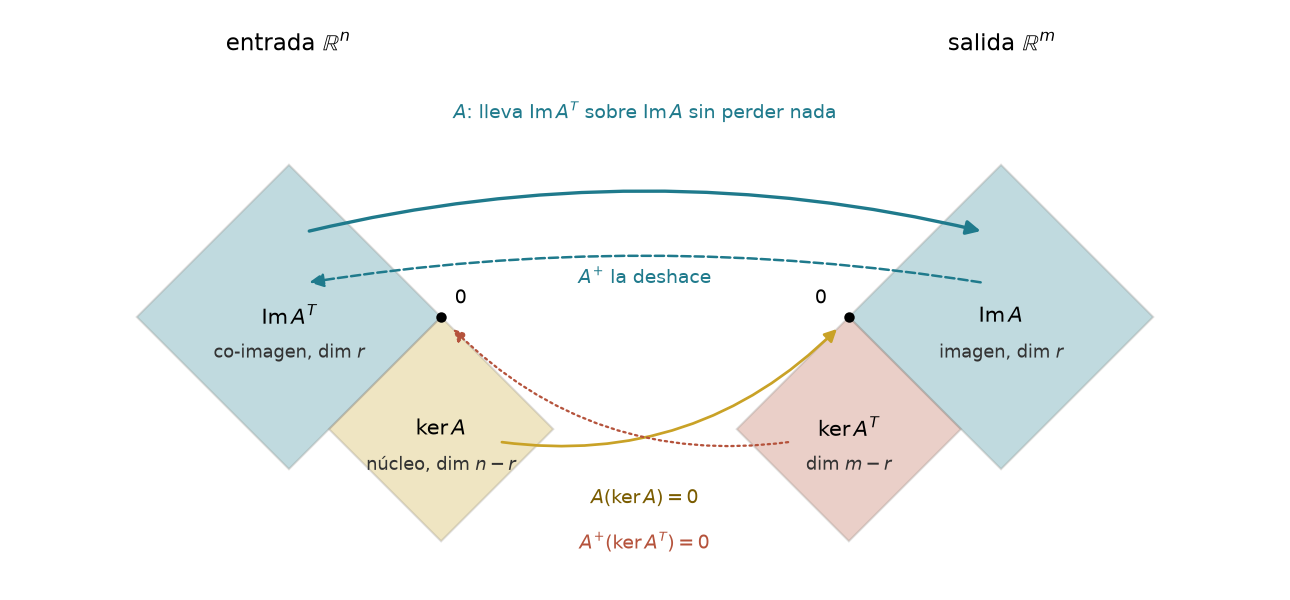
\includegraphics[width=.95\linewidth]{figuras/inversas/inv_cuatro_subespacios.png}
\caption{Los cuatro subespacios de una matriz \(A\) de \(m\times n\). En la
entrada, la co-imagen y el núcleo se cortan solo en el \(0\) y son perpendiculares; en la
salida, lo mismo la imagen y el espacio inaccesible. \(A\) manda el núcleo al \(0\) y lleva
la co-imagen sobre la imagen sin perder nada; \(A^{+}\) recorre ese camino al revés y manda
el espacio inaccesible al \(0\). Generada con
\texttt{apunte/scripts/cap11\_inversas\_pseudoinversa.py}.}
\label{fig:inv-cuatro-subespacios}
\end{figure}

\begin{ejemplo}[Los cuatro subespacios de una \(3\times2\) de rango \(2\)]\label{ej:cuatro-subespacios}
Sea \(A=\begin{pmatrix}1&0\\1&1\\1&2\end{pmatrix}\), la matriz de una recta \(y=b+ax\)
evaluada en \(x=0,1,2\) (incógnitas \((b,a)\)). Sus columnas \(a_1=(1,1,1)\) y
\(a_2=(0,1,2)\) no son paralelas: \(\operatorname{rango}A=2\), con \(m=3\), \(n=2\).
\begin{itemize}
  \item \textbf{Imagen} (dimensión \(2\)): el plano de \(\R^3\) generado por \(a_1\) y
  \(a_2\). Su normal es el cuña
  \(a_1\times a_2=(1\cdot2-1\cdot1,\ 1\cdot0-1\cdot2,\ 1\cdot1-1\cdot0)=(1,-2,1)\), y su
  ecuación es \(y_1-2y_2+y_3=0\).
  \item \textbf{Espacio inaccesible} (dimensión \(3-2=1\)): la recta de \((1,-2,1)\).
  Control: \(A^T(1,-2,1)^T=(1-2+1,\ 0-2+2)^T=(0,0)^T\).
  \item \textbf{Co-imagen} (dimensión \(2\)): las filas \((1,0)\), \((1,1)\), \((1,2)\)
  generan todo \(\R^2\).
  \item \textbf{Núcleo} (dimensión \(2-2=0\)): solo el \(0\); \(A^TA=\begin{pmatrix}3&3\\3&5\end{pmatrix}\)
  tiene determinante \(6\neq0\).
\end{itemize}
Lectura: tres mediciones \(y=(y_1,y_2,y_3)\) son compatibles con una recta si y solo si
\(y_1-2y_2+y_3=0\): si la segunda diferencia es nula (los tres puntos
equiespaciados están alineados). Cualquier otro \(y\) tiene una componente en la dirección
\((1,-2,1)\) que ninguna recta puede explicar.
\end{ejemplo}

\paragraph{Deshacer lo que se puede.} Volvé a la lámpara. La sombra no se puede deshacer del
todo, porque la altura de la varilla se perdió. Pero si alguien te muestra un punto de la mesa
y te pregunta de dónde vino, hay una respuesta razonable: de ese mismo punto, a altura cero,
sin inventar una altura que nadie midió. Y si te muestra un punto que \emph{no} está en la
mesa, flotando, lo razonable es bajarlo primero a la mesa, al punto más cercano, y después
contestar igual. Esa regla, aplicada a cualquier matriz, es la pseudoinversa \(A^{+}\) que anunciamos en
\enquote{La idea} (también llamada \emph{de Moore--Penrose}); se lee \enquote{\(A\) más}. Con la SVD
se arma como la inversa, pero \(\Sigma^{+}\) toma los recíprocos solo de los valores
singulares que no son cero: los estiramientos se deshacen, lo aplastado se deja en cero.

\begin{resultado}[Pseudoinversa de Moore--Penrose]
\[
  \boxed{\ A^{+}=V\,\Sigma^{+}\,U^T\ },\qquad
  \Sigma^{+}=\text{recíprocos de los }\sigma_i\neq0\text{, ceros donde había ceros}.
\]
Hecho geométrico: proyectar el término independiente sobre la imagen (descartar la parte
en el espacio inaccesible, que no se puede alcanzar) y deshacer solo la parte invertible;
si había núcleo, no inventar nada en la dirección aplastada (solución de norma mínima).
En \(\R\), la pseudoinversa de \(a=0\) es \(0\). Si \(A\) es cuadrada e invertible,
\(A^{+}=A^{-1}\); si \(A\) es alta (más filas que columnas) y sus columnas son
independientes, \(A^{+}=(A^TA)^{-1}A^T\), y \(x=A^{+}b\) resuelve las \emph{ecuaciones
normales} \(A^TAx=A^Tb\).
\end{resultado}

Las ecuaciones normales se llaman así porque piden que lo que sobra, \(b-Ax\), sea
\emph{normal} (perpendicular) a todas las columnas de \(A\); la
sección~\ref{sec:ecuaciones-normales} las deduce.

\paragraph{Sin inversa.} \(B=\begin{pmatrix}1&1\\1&1\end{pmatrix}\): \(\det B=0\), núcleo
\((1,-1)\), imagen la recta de \((1,1)\). \(Bx=(1,0)^T\) no tiene solución porque \((1,0)\)
no está en la imagen. SVD: \(\sigma_1=2\), \(\sigma_2=0\), \(u_1=v_1=\tfrac1{\sqrt2}(1,1)\);
entonces \(B^{+}=v_1\tfrac12u_1^T=\tfrac14\begin{pmatrix}1&1\\1&1\end{pmatrix}\) y
\(B^{+}(1,0)^T=(\tfrac14,\tfrac14)^T\): proyecta \((1,0)\) sobre la recta imagen (da
\((\tfrac12,\tfrac12)\)), deshace el estiramiento por \(2\) y no pone nada en la dirección
del núcleo. Otra que aplasta, la de la unidad \texttt{09}:
\(M=\begin{pmatrix}1&2\\2&4\end{pmatrix}\), rango \(1\), \(\sigma_1=5\),
\(u_1=v_1=\tfrac1{\sqrt5}(1,2)\), \(M^{+}=v_1\tfrac15u_1^T=\tfrac1{25}M\). Chequeo con
\(MM^{+}M=M\), una de las cuatro condiciones de Moore--Penrose
(definición~\ref{def:moore-penrose}): como \(M^2=5M\), \(M^3=25M\) y
\(M\cdot\tfrac1{25}M\cdot M=M\). Lo que \(M\) aplastó, la dirección \((2,-1)\), no vuelve:
\(M^{+}M=\tfrac15\begin{pmatrix}1&2\\2&4\end{pmatrix}\) es la proyección sobre \((1,2)\),
no la identidad.

\paragraph{Sistema sobredeterminado: una recta por tres puntos que no están alineados.}
Marcá en una hoja los puntos \((0,0)\), \((1,1)\) y \((2,3)\) y apoyá una regla sobre ellos.
¿Hay alguna posición de la regla que toque los tres? No: no están alineados.
Por \((0,0)\), \((1,1)\) y \((2,3)\) no pasa ninguna recta \(y=ax+b\): las tres ecuaciones no
se pueden cumplir a la vez. Lo que sí se puede es mover la regla hasta que los tres queden lo
más cerca posible. Dicho con la sombra de la lámpara: el vector \(y=(0,1,3)\) de las tres
alturas marcadas queda flotando fuera del plano de lo que una recta puede producir, y lo
bajamos a ese plano. Llamamos \(\hat x\) (se lee \enquote{\(x\) sombrero}) a la respuesta
elegida, la pendiente y la ordenada de la recta que mejor pasa; es la recta cuya salida
\(A\hat x\) es la proyección
ortogonal de \(y\) sobre el plano de las columnas de \(A\) (figura~\ref{fig:inv-proyeccion}).
Lo que sobra, \(r=y-A\hat x\), queda perpendicular a ese plano.
La cuenta completa, con las ecuaciones normales, lo que sobra y el proyector, es la del
ejemplo~\ref{ej:recta-cuatro-puntos}, con cuatro puntos.

\begin{figure}[htbp]
\centering
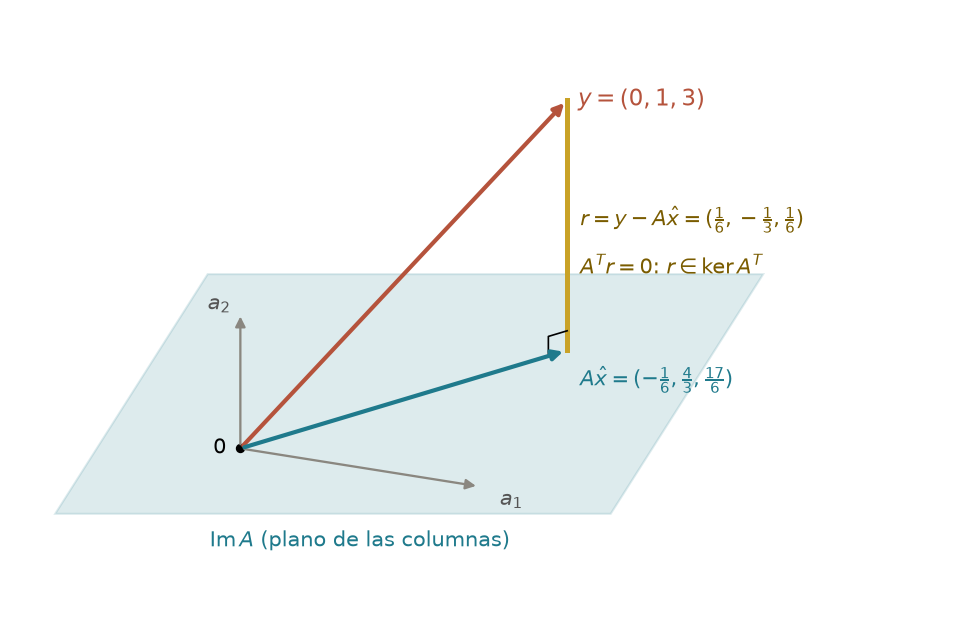
\includegraphics[width=.78\linewidth]{figuras/inversas/inv_proyeccion.png}
\caption{Esquema de la recta por tres puntos: \(y=(0,1,3)\) no está en el plano
\(\operatorname{im}A\) generado por las columnas \(a_1=(0,1,2)\) y \(a_2=(1,1,1)\). La
solución de mínimos cuadrados es la que da como salida la proyección ortogonal
\(A\hat x\); el residuo \(r\) es perpendicular al plano, es decir, está en \(\ker A^T\).
Generada con \texttt{apunte/scripts/cap11\_inversas\_pseudoinversa.py}.}
\label{fig:inv-proyeccion}
\end{figure}

\subsection{Sistemas sobredeterminados: las ecuaciones normales}\label{sec:ecuaciones-normales}

Cuando hay más ecuaciones que incógnitas, en general \(b\) no está en la imagen y \(Ax=b\) no
tiene solución. Elegimos entonces el \(\hat x\) cuya salida \(A\hat x\) es el punto de la
imagen más cercano a \(b\), su proyección ortogonal (figura~\ref{fig:inv-proyeccion}). Es la
regla apoyada sobre los puntos: de todas sus posiciones, nos quedamos con la que deja lo que
sobra perpendicular a todo lo que una recta puede producir. La proposición siguiente dice que
esa perpendicularidad es, justamente, la que da la distancia más chica, y la convierte en un
sistema cuadrado que siempre tiene solución.

\begin{proposicion}[Mínimos cuadrados y ecuaciones normales]\label{prop:ecuaciones-normales}
Sea \(A\) de \(m\times n\) y \(b\in\R^m\). Un vector \(\hat x\) minimiza
\(\lVert Ax-b\rVert\) si y solo si el residuo \(r=b-A\hat x\) es perpendicular a
\(\operatorname{im}A\), es decir, si y solo si
\[
  \boxed{\ A^TA\,\hat x=A^Tb\ } .
\]
Si las columnas de \(A\) son independientes (rango \(n\)), \(A^TA\) es invertible, la
solución es única y \(\hat x=A^{+}b\) con \(A^{+}=(A^TA)^{-1}A^T\).
\end{proposicion}

\begin{demostracion}
\(A^Tr=0\) dice que \(r\) es perpendicular a cada columna, o sea que \(r\in\ker A^T\). En
ese caso, para cualquier \(x\),
\(Ax-b=A(x-\hat x)-r\) es suma de un vector de la imagen y otro perpendicular a ella, y por
Pitágoras \(\lVert Ax-b\rVert^2=\lVert A(x-\hat x)\rVert^2+\lVert r\rVert^2\ge\lVert r\rVert^2\).
Recíprocamente, si \(A^Tr\neq0\), moverse un poco en la dirección \(A^Tr\) achica la
distancia. Si \(A^TAz=0\), entonces \(\lVert Az\rVert^2=z^TA^TAz=0\) y \(z\in\ker A\); con
columnas independientes \(z=0\) y \(A^TA\) es invertible.
\end{demostracion}

\begin{ejemplo}[Recta por cuatro puntos: ecuaciones normales, residuo y proyector]\label{ej:recta-cuatro-puntos}
Puntos \((0,1)\), \((1,2)\), \((2,2)\), \((3,4)\), recta \(y=ax+b\):
\[
  A=\begin{pmatrix}0&1\\1&1\\2&1\\3&1\end{pmatrix},\quad
  y=\begin{pmatrix}1\\2\\2\\4\end{pmatrix},\quad
  A^TA=\begin{pmatrix}14&6\\6&4\end{pmatrix},\quad
  A^Ty=\begin{pmatrix}18\\9\end{pmatrix}.
\]
Con \(\det A^TA=56-36=20\): \(a=\tfrac{4\cdot18-6\cdot9}{20}=0{,}9\) y
\(b=\tfrac{14\cdot9-6\cdot18}{20}=0{,}9\). La recta ajustada es \(y=0{,}9x+0{,}9\); sus
valores en los cuatro puntos son \((0{,}9;\ 1{,}8;\ 2{,}7;\ 3{,}6)\) y el residuo es
\[
  r=y-A\hat x=(0{,}1;\ 0{,}2;\ -0{,}7;\ 0{,}4),\qquad \lVert r\rVert^2=0{,}7 .
\]
Ortogonalidad: con la columna de unos, \(0{,}1+0{,}2-0{,}7+0{,}4=0\) (los residuos suman
cero); con la columna de las \(x\), \(0+0{,}2-1{,}4+1{,}2=0\). La pseudoinversa y el
proyector sobre la imagen son
\[
  A^{+}=(A^TA)^{-1}A^T=\frac1{20}\begin{pmatrix}-6&-2&2&6\\14&8&2&-4\end{pmatrix},\qquad
  P=AA^{+}=\frac1{10}\begin{pmatrix}7&4&1&-2\\4&3&2&1\\1&2&3&4\\-2&1&4&7\end{pmatrix}.
\]
\setlength{\emergencystretch}{1em}%
\(P\) es simétrica, \(P^2=P\) y su traza vale \(2=\operatorname{rango}A\); \(Py\) da los
valores ajustados y \((I-P)y=(0{,}1;\ 0{,}2;\ -0{,}7;\ 0{,}4)\) da el residuo. Verificado
numéricamente por dos caminos, resolviendo el sistema y multiplicando por la pseudoinversa:
\((0{,}9;\ 0{,}9)\).
\end{ejemplo}

\subsection{Sistemas subdeterminados: la solución de norma mínima}\label{sec:norma-minima}

Suponé que de dos números solo sabés que el primero más el doble del segundo da \(5\).
¿Cuáles son? Pueden ser \(5\) y \(0\), \(3\) y \(1\), \(1\) y \(2\), y infinitos pares más:
falta información. Si hay que dar una sola respuesta, ¿cuál es la más honesta? La que no
agrega nada que los datos no digan: la más corta, la más cercana al origen
(figura~\ref{fig:inv-norma-minima}). Pasa lo mismo con las alturas de \enquote{La idea}: si
solo se midió cuánto más alto está un punto que otro, ninguna medición decide cuánto suben o
bajan los dos juntos, y lo honesto es no inventarlo.

Con menos ecuaciones independientes que incógnitas pasa lo opuesto: si \(A\) de \(m\times n\)
tiene rango \(m<n\), toda \(b\) está en la imagen, pero a cualquier solución se le puede sumar
un vector del núcleo. El conjunto de
soluciones es un subespacio afín, paralelo a \(\ker A\) (definición~\ref{def:subespacio}).
De todas, una sola es perpendicular al núcleo: la que no tiene ninguna componente
\enquote{inventada} en las direcciones que \(A\) no ve. La llamamos \(x^{+}\), porque es la
que da la pseudoinversa, y es la más corta: cualquier otra es ella más un pedazo de núcleo,
perpendicular, y por Pitágoras más larga.

\begin{figure}[htbp]
\centering
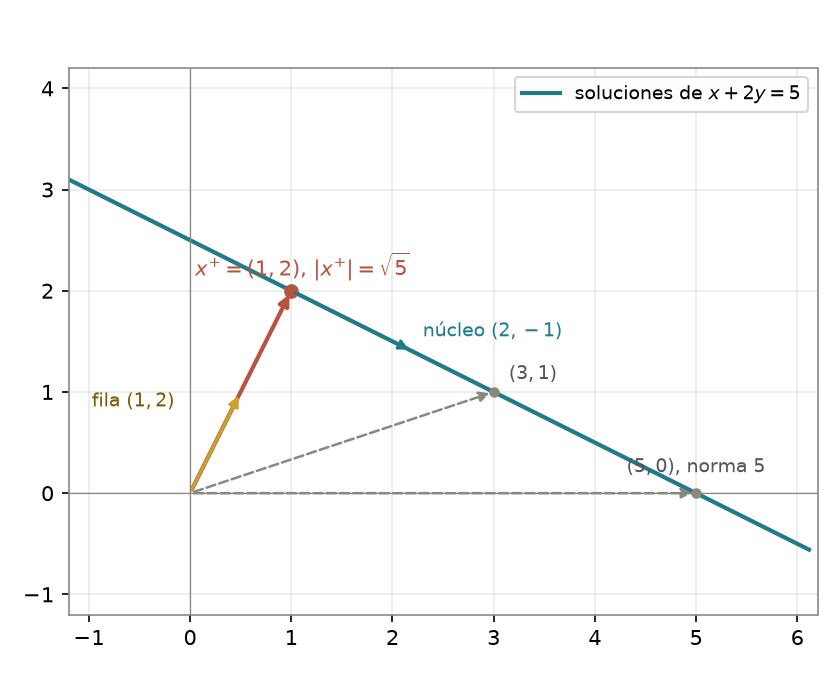
\includegraphics[width=.62\linewidth]{figuras/inversas/inv_norma_minima.png}
\caption{Las soluciones de \(x+2y=5\) forman una recta paralela al núcleo \((2,-1)\). La de
norma mínima, \(x^{+}=(1,2)\), es el pie de la perpendicular desde el origen y apunta en la
dirección de la fila \((1,2)\), es decir, está en la co-imagen. Otras soluciones, como
\((3,1)\) o \((5,0)\), son más largas. Generada con
\texttt{apunte/scripts/cap11\_inversas\_pseudoinversa.py}.}
\label{fig:inv-norma-minima}
\end{figure}

\begin{proposicion}[Solución de norma mínima]\label{prop:norma-minima}
Si \(A\) de \(m\times n\) tiene filas independientes (rango \(m\)), \(AA^T\) es invertible y
\[
  \boxed{\ x^{+}=A^{+}b,\qquad A^{+}=A^T(AA^T)^{-1}\ }
\]
es la única solución de \(Ax=b\) que está en \(\operatorname{im}A^T\), y la de menor norma.
\end{proposicion}

\begin{demostracion}
\(Ax^{+}=AA^T(AA^T)^{-1}b=b\), y \(x^{+}=A^Tw\) con \(w=(AA^T)^{-1}b\) es combinación de
las filas. Cualquier otra solución es \(x=x^{+}+k\) con \(k\in\ker A\), perpendicular a
\(x^{+}\) por la proposición~\ref{prop:cuatro-subespacios}; por Pitágoras
\(\lVert x\rVert^2=\lVert x^{+}\rVert^2+\lVert k\rVert^2\). \(AA^T\) es invertible por el
mismo argumento de la proposición~\ref{prop:ecuaciones-normales}, aplicado a \(A^T\).
\end{demostracion}

\begin{ejemplo}[Norma mínima de un sistema \(2\times3\) y las condiciones de Moore--Penrose]\label{ej:norma-minima}
Sean \(A=\begin{pmatrix}1&1&1\\1&-1&0\end{pmatrix}\) y \(b=(3,1)\). Las filas son
perpendiculares, así que \(AA^T=\operatorname{diag}(3,2)\) y
\[
  A^{+}=A^T(AA^T)^{-1}=\frac16\begin{pmatrix}2&3\\2&-3\\2&0\end{pmatrix},\qquad
  x^{+}=A^{+}b=(1{,}5;\ 0{,}5;\ 1),\qquad \lVert x^{+}\rVert^2=3{,}5 .
\]
Control: \(Ax^{+}=(1{,}5+0{,}5+1;\ 1{,}5-0{,}5)=(3,1)\). El núcleo es la recta del cuña de
las filas, \((1,1,1)\times(1,-1,0)=(1,1,-2)\), y \(x^{+}\cdot(1,1,-2)=1{,}5+0{,}5-2=0\): la
solución de norma mínima no tiene componente en el núcleo. Otra solución, por ejemplo
\(x^{+}+\tfrac12(1,1,-2)=(2,1,0)\), cumple igual \(Ax=b\) pero tiene
\(\lVert x\rVert^2=5=3{,}5+\tfrac14\cdot6\).

Las cuatro condiciones de Moore--Penrose se verifican a mano:
\[
  AA^{+}=I_2,\qquad
  A^{+}A=\frac16\begin{pmatrix}5&-1&2\\-1&5&2\\2&2&2\end{pmatrix}.
\]
Las dos son simétricas; \(AA^{+}A=I_2A=A\) y \(A^{+}AA^{+}=A^{+}I_2=A^{+}\). El script
lo confirma con error máximo \(5{,}6\cdot10^{-17}\), y \(V\Sigma^{+}U^T\) (con
\(\sigma_1=\sqrt3\), \(\sigma_2=\sqrt2\)) coincide con la pseudoinversa que calcula NumPy.
\(A^{+}A\) es el proyector sobre la co-imagen: deja fijas las filas de \(A\) y manda
\((1,1,-2)\) al cero.
\end{ejemplo}

\subsection{Simulaciones}

\unidadInteractiva{11_cuatro_problemas}{Cuatro problemas: regresión, círculos, Procrustes, regresión total}{Verificá: en el problema «(a) recta de ajuste» mové el ruido y comprobá que \(A^Tr\) sigue dando \((0,0)\): el residuo es perpendicular a la columna de las \(x\) y a la de unos, como en el ejemplo~\ref{ej:recta-cuatro-puntos}.}

\unidadInteractiva{09_cambio_de_base_svd}{Cambio de base, SVD e inversas}{Verificá: en el caso «aplastante [[1, 2], [2, 4]]» comprobá que \(\sigma_2=0\), que no hay inversa, y que en la sección de cuentas \(P^{+}=P/25\) cumple \(PP^{+}P=P\).}

\section{En profundidad}

\subsection{Demostración de la fórmula de la adjugada}\label{sec:inv-demostraciones}

Demostramos acá la proposición~\ref{prop:adjugada-inversa}: la adjugada, puesta al lado de
\(A\), deja \(\det A\) en la diagonal y ceros fuera de ella. La idea es la de los ejemplos en
\(2\times2\) y \(3\times3\): cada columna de la adjugada es perpendicular a todas las filas de
\(A\) salvo una.

\begin{demostracion}
Sea \(C_{ij}\) el cofactor \((i,j)\). La entrada \((i,k)\) de \(A\,\operatorname{adj}(A)\) es
\(\sum_j a_{ij}C_{kj}\). Si \(k=i\), es \(\sum_j a_{ij}C_{ij}\), el desarrollo de \(\det A\)
por la fila \(i\) (el desarrollo por menores del ejemplo~\ref{ej:det-volumen}, que vale por
cualquier fila): da \(\det A\). Si \(k\neq i\), sea \(A'\) la matriz que resulta de
reemplazar la fila \(k\) de \(A\) por la fila \(i\). Los cofactores \(C_{kj}\) no dependen
de la fila \(k\), así que son los mismos en \(A\) y en \(A'\), y \(\sum_j a_{ij}C_{kj}\) es el
desarrollo de \(\det A'\) por la fila \(k\). Pero \(A'\) tiene dos filas iguales, y su
determinante es cero: intercambiar esas dos filas no cambia la matriz y, como el
determinante es alternado (sección~\ref{sec:exterior}), le cambia el signo, así que
\(\det A'=-\det A'\). Por lo tanto \(A\,\operatorname{adj}(A)=(\det A)\,I\). Con el
desarrollo por columnas el mismo argumento da \(\operatorname{adj}(A)\,A=(\det A)\,I\): la
entrada \((i,k)\) es \(\sum_j C_{ji}a_{jk}\), el desarrollo por la columna \(i\) de la
matriz que tiene la columna \(k\) de \(A\) en el lugar de la \(i\). Si \(\det A\neq0\),
dividiendo por \(\det A\) queda \(A\,\tfrac{\operatorname{adj}(A)}{\det A}=
\tfrac{\operatorname{adj}(A)}{\det A}\,A=I\).
\end{demostracion}

\subsection{El caso general: pseudoinversa por SVD}\label{sec:pinv-svd}

¿Y si pasan las dos cosas a la vez, que la matriz aplaste alguna dirección y que además no
alcance toda la salida? Es la lámpara sobre la mesa: se pierde la altura de la varilla y
ninguna sombra queda flotando. Las dos fórmulas anteriores piden rango completo: por columnas, \((A^TA)^{-1}A^T\); por
filas, \(A^T(AA^T)^{-1}\). Cuando el rango es menor que \(m\) y que \(n\) (hay a la vez
espacio inaccesible y núcleo) ninguna de las dos sirve, porque \(A^TA\) y \(AA^T\) son
singulares. La SVD resuelve el caso general con \(A^{+}=V\Sigma^{+}U^T\), y \(A^{+}b\)
combina las dos virtudes: su salida
\(AA^{+}b\) es la proyección de \(b\) sobre la imagen (la mejor aproximación) y, entre todos
los \(x\) con esa salida, es el de norma mínima.

¿Cómo se reconoce una pseudoinversa sin volver a calcular la SVD? Con cuatro condiciones que
solo piden multiplicar y transponer.

\begin{definicion}[Condiciones de Moore--Penrose]\label{def:moore-penrose}
Una matriz \(X\) de \(n\times m\) es \emph{pseudoinversa} de \(A\) (de \(m\times n\)) si
\[
  \text{(1) } AXA=A,\qquad \text{(2) } XAX=X,\qquad
  \text{(3) } (AX)^T=AX,\qquad \text{(4) } (XA)^T=XA .
\]
\end{definicion}

\begin{proposicion}[Existencia y unicidad de la pseudoinversa]\label{prop:moore-penrose}
\(X=V\Sigma^{+}U^T\) cumple las cuatro condiciones, y es la única matriz que las cumple.
\end{proposicion}

\begin{demostracion}
Con \(A=U\Sigma V^T\) y \(U,V\) ortogonales, \(AX=U\Sigma\Sigma^{+}U^T\) y
\(XA=V\Sigma^{+}\Sigma V^T\); \(\Sigma\Sigma^{+}\) y \(\Sigma^{+}\Sigma\) son diagonales con
unos donde \(\sigma_i\neq0\) y ceros en el resto, así que (3) y (4) se cumplen, y
\(\Sigma\Sigma^{+}\Sigma=\Sigma\), \(\Sigma^{+}\Sigma\Sigma^{+}=\Sigma^{+}\) dan (1) y (2).
Unicidad: si \(X\) e \(Y\) cumplen las cuatro, usando alternadamente (2), (3) o (4) y (1),
\[
  X=XAX=X(AX)^T=XX^TA^T=XX^T(AYA)^T=X(AX)^T(AY)^T=XAXAY=XAY,
\]
\[
  Y=YAY=(YA)^TY=A^TY^TY=(AXA)^TY^TY=(XA)^T(YA)^TY=XAYAY=XAY,
\]
y entonces \(X=Y\).
\end{demostracion}

Las cuatro condiciones permiten verificar una pseudoinversa sin recalcularla, como en el
ejemplo~\ref{ej:norma-minima} y en la red sin alturas fijas de la
sección~\ref{sec:aplicacion-nivelacion}.

\subsection{Proyectores: lo que se explica y lo que sobra}\label{sec:proyectores}

Las condiciones (1) y (3) dicen que \(P=AA^{+}\) es simétrica y cumple
\(P^2=AA^{+}AA^{+}=AA^{+}=P\): es la \emph{proyección ortogonal} sobre
\(\operatorname{im}A\). Su complemento \(I-P\) proyecta sobre \(\ker A^T\). Cuando medimos de
más,
\[
  b=\underbrace{Pb}_{\text{lo que el modelo explica}}+\underbrace{(I-P)b}_{\text{residuo}},
\]
dos vectores perpendiculares. Del lado de la entrada, \(A^{+}A\) proyecta sobre la co-imagen
e \(I-A^{+}A\) sobre el núcleo; por eso todas las mejores aproximaciones se escriben
\[
  x=A^{+}b+(I-A^{+}A)\,z,\qquad z\in\R^n\ \text{arbitrario},
\]
y \(A^{+}b\) es la que corresponde a no agregar nada en el núcleo. La traza de un proyector
es la dimensión del subespacio sobre el que proyecta: \(\operatorname{tr}P=\operatorname{rango}A\) y
\(\operatorname{tr}(I-P)=m-\operatorname{rango}A\), la cantidad de \emph{grados de libertad}: cuántas mediciones
sobran respecto de las estrictamente necesarias. Ese
número, \(m-\operatorname{rango}A\), es el que divide a \(v^Tv\), la suma de los cuadrados de lo que sobra, en el
desvío estándar de la sección siguiente.

\begin{idea}[Aproximar es partir el dato en dos piezas perpendiculares]
Las incógnitas se leen de la proyección \(Pb\); la calidad de la medición, del resto
perpendicular \((I-P)b\).
\end{idea}

\subsection{Aplicación topográfica: las alturas de cuatro puntos}\label{sec:aplicacion-nivelacion}

Hay cuatro puntos en un terreno y medimos cuánto sube el terreno de uno a otro por seis
caminos, más de los que hacen falta. Las medidas no cierran exacto: si se sube de \(A\) a
\(B\), de \(B\) a \(C\) y se vuelve de \(C\) a \(A\), lo subido y lo bajado deberían
compensarse, y sobran unos milímetros. Conocemos la altura de uno de los puntos y queremos la
de los otros tres. Es la situación de \enquote{La idea}, con un punto más y tres caminos más.

\begin{idea}[Esto lo vas a usar en Topografía]
La altura de un punto sobre una referencia elegida se llama \emph{cota}, y la diferencia de
altura entre dos puntos, \emph{desnivel}; lo mide un instrumento que dice cuánto más alto está
un punto que otro. Medir así, tramo por tramo, es \emph{nivelación}, y un conjunto de puntos
unidos por mediciones de ese tipo, con más de las necesarias, forma una \emph{red}. Repartir lo que no cierra
entre las mediciones, para obtener alturas compatibles con todas, es buscar la mejor
aproximación de la sección~\ref{sec:ecuaciones-normales}.
\end{idea}

Llamamos \(A\), \(B\), \(C\) y \(D\) a los cuatro puntos y \(H_A\), \(H_B\), \(H_C\), \(H_D\)
a sus alturas. La de \(A\) es conocida y queda fija, \(H_A=100{,}000\) m, y buscamos las de
\(B\), \(C\), \(D\). Se midieron seis tramos; llamamos \(\ell_k\) a lo que se midió en el tramo
\(k\): la altura del punto de llegada menos la del punto de salida
(figura~\ref{fig:inv-red-nivelacion}).

\begin{figure}[htbp]
\centering
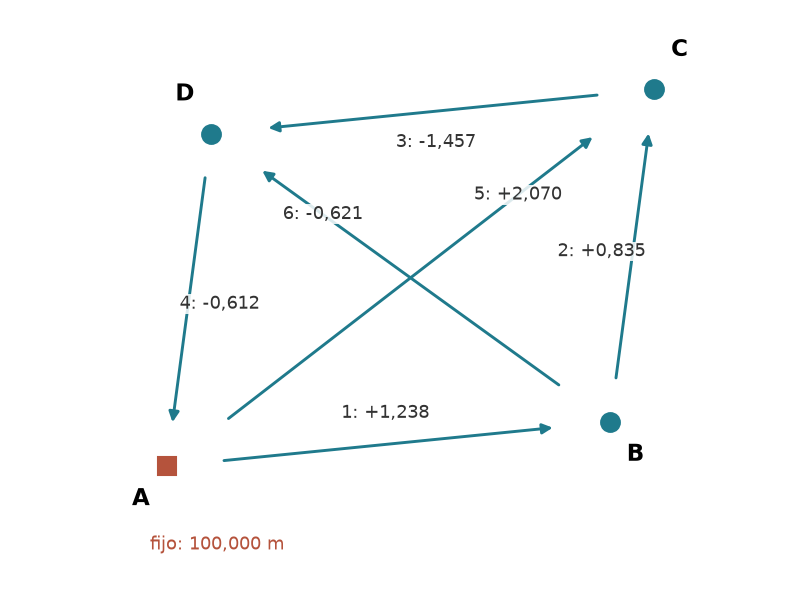
\includegraphics[width=.6\linewidth]{figuras/inversas/inv_red_nivelacion.png}
\caption{Red de nivelación con un punto fijo \(A\) y tres incógnitas. Cada flecha es un
tramo nivelado, de la salida a la llegada, con su número y su desnivel medido en metros.
Generada con \texttt{apunte/scripts/cap11\_inversas\_pseudoinversa.py}.}
\label{fig:inv-red-nivelacion}
\end{figure}

\begin{center}
\small
\begin{tabular}{clr}
\toprule
tramo & de \(\to\) a & \(\ell_k\) (m)\\
\midrule
1 & \(A\to B\) & \(1{,}238\)\\
2 & \(B\to C\) & \(0{,}835\)\\
3 & \(C\to D\) & \(-1{,}457\)\\
4 & \(D\to A\) & \(-0{,}612\)\\
5 & \(A\to C\) & \(2{,}070\)\\
6 & \(B\to D\) & \(-0{,}621\)\\
\bottomrule
\end{tabular}
\end{center}

\paragraph{Los cierres no son nulos.} Si se sale de un punto y se vuelve a él, lo subido
tiene que igualar lo bajado: en un circuito cerrado la suma de las diferencias medidas
debería ser cero, y lo que da en cambio se llama \emph{cierre} del circuito. Con los datos: \(A\to B\to C\to A\) da \(1{,}238+0{,}835-2{,}070=+3\) mm;
\(A\to C\to D\to A\), \(+1\) mm; \(B\to C\to D\to B\), \(-1\) mm; \(A\to B\to D\to A\),
\(+5\) mm. Seis ecuaciones, tres incógnitas: el sistema es incompatible y buscamos la mejor
aproximación, como en la sección~\ref{sec:ecuaciones-normales}.

\paragraph{Matriz de diseño.} La matriz \(A\) del sistema se llama en este contexto
\emph{matriz de diseño}: dice qué tramos se midieron y entre qué puntos. Con
\(x=(H_B,H_C,H_D)\), cada tramo da una ecuación
\(H_{\text{llegada}}-H_{\text{salida}}=\ell_k\); la altura conocida de \(A\) pasa al término
independiente:
\[
  A=\begin{pmatrix}1&0&0\\-1&1&0\\0&-1&1\\0&0&-1\\0&1&0\\-1&0&1\end{pmatrix},\qquad
  b=\begin{pmatrix}\ell_1+H_A\\ \ell_2\\ \ell_3\\ \ell_4-H_A\\ \ell_5+H_A\\ \ell_6\end{pmatrix}
  =\begin{pmatrix}101{,}238\\0{,}835\\-1{,}457\\-100{,}612\\102{,}070\\-0{,}621\end{pmatrix}.
\]
Cada fila tiene un \(+1\) en el punto de llegada y un \(-1\) en el de salida (salvo cuando
ese punto es \(A\)).

\paragraph{Ecuaciones normales.}
\[
  A^TA=\begin{pmatrix}3&-1&-1\\-1&3&-1\\-1&-1&3\end{pmatrix},\qquad
  A^Tb=\begin{pmatrix}101{,}024\\104{,}362\\98{,}534\end{pmatrix},\qquad
  (A^TA)^{-1}=\frac18\begin{pmatrix}4&2&2\\2&4&2\\2&2&4\end{pmatrix}.
\]
La diagonal de \(A^TA\) cuenta los tramos que concurren a cada punto (tres en todos los casos)
y los \(-1\) indican qué pares están vinculados por un tramo; \(\det A^TA=16\). Las alturas
que resultan son
\[
  \boxed{\ H_B=101{,}2360\ \text{m},\quad H_C=102{,}0705\ \text{m},\quad H_D=100{,}6135\ \text{m}\ } .
\]

\paragraph{Correcciones y cierres.} Llamamos \(v\) a la corrección de cada tramo,
\(v=A\hat x-b\): lo que el tramo sube según las alturas que resultan, menos lo que se midió.
En milímetros:
\[
  v=(-2{,}0;\ -0{,}5;\ 0{,}0;\ -1{,}5;\ +0{,}5;\ -1{,}5),\qquad v^Tv=9\ \text{mm}^2,
  \qquad A^Tv=0 .
\]
Las diferencias corregidas, \(\ell_k+v_k\), son \(1{,}2360\); \(0{,}8345\); \(-1{,}4570\);
\(-0{,}6135\); \(2{,}0705\); \(-0{,}6225\) m, y \emph{cierran exactamente} en cada circuito:
en \(A\to B\to C\to A\), \(1{,}2360+0{,}8345-2{,}0705=0\). Dicho con las correcciones: en cada
circuito suman lo mismo que el cierre medido, cambiado de signo
(\(v_1+v_2-v_5=-2{,}0-0{,}5-0{,}5=-3\) mm; en los otros tres circuitos, \(-1\), \(+1\) y
\(-5\) mm). Hecho geométrico: \(v\) es la componente de las mediciones que está fuera de la
imagen, y la imagen está formada justamente por las listas de diferencias que cierran. De
los cuatro circuitos solo tres son independientes (\(6-3=3\), la dimensión de
\(\ker A^T\)): los vectores de circuito generan el espacio inaccesible.

\paragraph{Precisión.} ¿Cuánto confiar en las alturas que resultan? Lo dicen las
correcciones: si son chicas, las mediciones eran buenas. El número que lo resume es
\(\sigma_0\), el \emph{desvío estándar de la unidad de peso}, que mide cuánto se equivoca,
típicamente, una medición. Usa los \(n-u=6-3=3\) grados
de libertad (acá \(n\) cuenta las mediciones y \(u\) las incógnitas):
\[
  \sigma_0=\sqrt{\frac{v^Tv}{n-u}}=\sqrt{\frac{9}{3}}\ \text{mm}=1{,}732\ \text{mm},
\]
y la precisión de cada altura es \(\sigma_0\sqrt{(A^TA)^{-1}_{ii}}\). Los tres elementos
diagonales de \((A^TA)^{-1}\) valen \(\tfrac12\), así que
\(\sigma_{H_B}=\sigma_{H_C}=\sigma_{H_D}=1{,}732\cdot0{,}7071=1{,}225\) mm. Que las tres
coincidan refleja la simetría de la red: cada punto está unido a los otros tres.

\paragraph{Sin ninguna altura conocida.} ¿Y si no conocemos la altura de ninguno de los
cuatro puntos?
Imaginá que solo tenés las seis mediciones de cuánto sube el terreno de un punto a otro. Es el
segundo caso de \enquote{La idea}: las mediciones dicen cuánto más alto está cada punto que
los otros, pero no dónde está el conjunto. Un conjunto de puntos unidos por mediciones, sin
ninguna altura fija, se llama \emph{red libre}. Sin ninguna altura fija, las incógnitas son
las cuatro,
\(x=(H_A,H_B,H_C,H_D)\), y la matriz de diseño, que llamamos \(A_\ell\), es de \(6\times4\),
con una columna más para \(A\):
\[
  A_\ell=\begin{pmatrix}-1&1&0&0\\0&-1&1&0\\0&0&-1&1\\1&0&0&-1\\-1&0&1&0\\0&-1&0&1\end{pmatrix},
  \qquad
  A_\ell^TA_\ell=\begin{pmatrix}3&-1&-1&-1\\-1&3&-1&-1\\-1&-1&3&-1\\-1&-1&-1&3\end{pmatrix}.
\]
Cada fila suma cero, así que \(A_\ell(1,1,1,1)^T=0\): el núcleo es la recta de
\((1,1,1,1)\). Subir todos los puntos lo mismo no cambia ninguna diferencia de altura: las
mediciones no pueden decidir la altura absoluta del conjunto. El rango es \(3\) y
\(A_\ell^TA_\ell\) es
singular (\(\det=0\); los valores singulares de \(A_\ell\) son \(2\), \(2\), \(2\) y \(0\)),
de modo que
las ecuaciones normales tienen infinitas soluciones. La pseudoinversa elige la de norma
mínima:
\[
  x^{+}=A_\ell^{+}\,\ell=(-0{,}9800;\ 0{,}2560;\ 1{,}0905;\ -0{,}3665)\ \text{m},
\]
cuyas componentes suman cero: \(x^{+}\) es perpendicular al núcleo. Esas \enquote{alturas} no tienen
sentido físico por sí solas (están referidas al promedio de los cuatro puntos), pero sus
diferencias sí. Trasladándolas por \(t=100{,}9800\) m en la dirección del núcleo, para que
\(H_A=100{,}000\), quedan \(101{,}2360\), \(102{,}0705\) y \(100{,}6135\) m: las mismas alturas
que con \(A\) conocido. Las correcciones y las diferencias corregidas son idénticas en los dos
enfoques, porque \(A\) y \(A_\ell\) tienen la misma imagen (la columna de \(A\) en
\(A_\ell\) es menos la suma de las otras tres) y por lo tanto el mismo proyector
\(P=AA^{+}=A_\ell A_\ell^{+}\).

Hecho geométrico: el \emph{datum}, la referencia desde la que se cuentan las alturas, vive en
el núcleo. Elegir la altura de un punto, o fijar el
promedio, es elegir un punto sobre la recta de soluciones \(x^{+}+t(1,1,1,1)\); las
diferencias de altura, la imagen y lo que sobra no dependen de esa elección. Se comprueban las
cuatro condiciones de Moore--Penrose para \(A_\ell^{+}\) (error máximo
\(4{,}4\cdot10^{-16}\)) y que \(A_\ell^{+}A_\ell=I-\tfrac14\,\mathbf 1\mathbf 1^T\), con
\(\mathbf 1=(1,1,1,1)\) el vector de unos: es el
proyector que quita a cada lista de alturas su promedio.

\section{Ejercicios con solución}

\begin{ejercicio}\label{ex:inv-2x2-rotacion}
(a) Calculá la inversa de \(M=\begin{pmatrix}3&1\\5&2\end{pmatrix}\) y verificala.
(b) Escribí \(R(30^\circ)^{-1}\) sin calcular ningún determinante y explicá por qué.
\end{ejercicio}
\solucion{(a) \(\det M=6-5=1\), así que
\(M^{-1}=\begin{pmatrix}2&-1\\-5&3\end{pmatrix}\). Control: primera fila de \(M\) por las
columnas de \(M^{-1}\): \(6-5=1\), \(-3+3=0\); segunda fila: \(10-10=0\), \(-5+6=1\).
(b) \(R(30^\circ)^{-1}=R(-30^\circ)=R(30^\circ)^T
=\begin{pmatrix}\cos30^\circ&\sin30^\circ\\-\sin30^\circ&\cos30^\circ\end{pmatrix}
\approx\begin{pmatrix}0{,}866&0{,}5\\-0{,}5&0{,}866\end{pmatrix}\): las columnas de una
rotación son ortonormales, así que \(R^TR=I\).}

\begin{ejercicio}\label{ex:inv-cuatro-subespacios}
Encontrá una base de cada uno de los cuatro subespacios de
\(B=\begin{pmatrix}1&2&3\\2&4&6\end{pmatrix}\), verificá las ortogonalidades y las
dimensiones, y comprobá que \(B^{+}=\tfrac1{70}B^T\).
\end{ejercicio}
\solucion{La segunda fila es el doble de la primera: \(\operatorname{rango}B=1\), con \(m=2\), \(n=3\).
Imagen: \(\langle(1,2)\rangle\), dimensión \(1\); espacio inaccesible:
\(\langle(2,-1)\rangle\), dimensión \(2-1=1\), y en efecto \(B^T(2,-1)^T=0\). Co-imagen:
\(\langle(1,2,3)\rangle\), dimensión \(1\); núcleo: \(\langle(2,-1,0),\ (3,0,-1)\rangle\),
dimensión \(3-1=2\); ambos vectores dan \(B v=0\) y son perpendiculares a \((1,2,3)\)
(\(2-2+0=0\), \(3+0-3=0\)). Como \(B=uv^T\) con \(u=(1,2)\) y \(v=(1,2,3)\), la SVD tiene un
solo valor singular, \(\sigma_1=\lVert u\rVert\lVert v\rVert=\sqrt{5\cdot14}=\sqrt{70}\), y
\(B^{+}=\tfrac{v}{\lVert v\rVert}\tfrac1{\sqrt{70}}\tfrac{u^T}{\lVert u\rVert}=\tfrac{vu^T}{70}
=\tfrac1{70}B^T\).}

\begin{ejercicio}\label{ex:inv-media}
Una distancia se midió tres veces: \(125{,}432\), \(125{,}438\) y \(125{,}429\) m.
Planteá el ajuste como un sistema \(Ax=b\) de \(3\times1\) y calculá \(A^{+}\), el valor
ajustado, los residuos, \(\sigma_0\) y la precisión del valor ajustado.
\end{ejercicio}
\solucion{\(A=(1,1,1)^T\), \(A^TA=3\), \(A^{+}=\tfrac13(1,1,1)\): la pseudoinversa es el
promedio. \(\hat d=\tfrac13(125{,}432+125{,}438+125{,}429)=125{,}433\) m. Residuos
\(v=\hat d-b=(+1;\ -5;\ +4)\) mm, que suman cero (son perpendiculares a la columna de unos).
\(v^Tv=42\) mm\(^2\), \(n-u=2\), \(\sigma_0=\sqrt{42/2}=4{,}583\) mm, y
\(\sigma_{\hat d}=\sigma_0\sqrt{(A^TA)^{-1}}=4{,}583/\sqrt3=2{,}646\) mm.}

\begin{ejercicio}\label{ex:inv-norma-minima}
Hallá la solución de norma mínima de la ecuación \(x+2y+2z=9\) y comparala con la solución
\((9,0,0)\). ¿Qué forma tiene el conjunto de todas las soluciones?
\end{ejercicio}
\solucion{\(A=(1\ 2\ 2)\), \(AA^T=9\), \(A^{+}=\tfrac19(1,2,2)^T\), \(x^{+}=A^{+}\cdot9=(1,2,2)\),
con \(\lVert x^{+}\rVert=3\); control: \(1+4+4=9\). \((9,0,0)\) también es solución pero
tiene norma \(9\). El conjunto de soluciones es el plano afín \(x+2y+2z=9\), paralelo al
núcleo (el plano \(x+2y+2z=0\)); \(x^{+}\) es el pie de la perpendicular desde el origen y
apunta en la dirección de la normal \((1,2,2)\), que genera la co-imagen. Su norma, \(3\), es
la distancia del origen al plano: \(9/\lVert(1,2,2)\rVert=9/3\).}

\begin{ejercicio}\label{ex:inv-proyector}
Para la matriz \(A\) del ejemplo~\ref{ej:cuatro-subespacios}, calculá \(P=AA^{+}\) e
\(I-P\), verificá que \(I-P=\tfrac16\,nn^T\) con \(n=(1,-2,1)\) y descomponé
\(y=(1,0,2)\) en una parte explicada por una recta y un residuo.
\end{ejercicio}
\solucion{\(A^TA=\begin{pmatrix}3&3\\3&5\end{pmatrix}\), y
\(P=A(A^TA)^{-1}A^T=\tfrac16\begin{pmatrix}5&2&-1\\2&2&2\\-1&2&5\end{pmatrix}\), de traza
\(2\). \(I-P=\tfrac16\begin{pmatrix}1&-2&1\\-2&4&-2\\1&-2&1\end{pmatrix}=\tfrac16\,nn^T\): la
proyección sobre la recta del espacio inaccesible, con \(\lVert n\rVert^2=6\). Para
\(y=(1,0,2)\): \(Py=(0{,}5;\ 1;\ 1{,}5)\), alineados (la recta \(y=0{,}5+0{,}5x\)), y
\((I-P)y=(0{,}5;\ -1;\ 0{,}5)\), un múltiplo de \(n\), perpendicular a las dos columnas.}
